\begin{chapter}{\label{cha:nonequib}Critical velocity at finite temperature}
  \section{Introduction}
A defining feature of superfluids is the spontaneous formation of excitations when the flow exceeds a critical velocity relative to some obstacle or boundary, marking the breakdown of superfluid transport and the onset of dissipation.  This can be understood in terms of the Landau criterion, which predicts excitations when the local fluid velocity exceeds $v_{\rm L} = \textrm{min} [E(p)/p]$, where $p$ is the momentum of elementary excitations and $E(p)$ their energy \cite{NozieresPines}.  In weakly-interacting atomic Bose-Einstein condensates,  $v_{\rm L}=c$, the speed of sound.  The breakdown of superfluidity has been experimentally probed by introducing a localized repulsive obstacle, engineered via the repulsive force generated by focussed blue-detuned laser beam, and moving the condensate relative to the obstacle \cite{Neely,kwon_moon_14,kwon_2015a,kwon_2015b,Raman,Onofrio,Inouye,desbuquois_2012}.  This has enabled measurement of the critical velocity and the direct observation of the ensuing excitations, that is, pairs of quantized vortex lines with opposite polarity.  In flattened condensates, this scenario is providing a route to engineer states of two-dimensional quantum turbulence \cite{Neely,kwon_moon_14}.  This scenario is also providing insight into the deep link between quantum fluids and their classical counterparts, where it has been predicted that the wake of quantized vortices produced downstream of the obstacle can collectively mimick the classical wakes, including the B{\' e}rnard-von K{\'a} rm{\' a}n vortex street \cite{saito_2010,stagg_2014}.  



The motion of an obstacle in the zero-temperature Bose gas, described by the Gross-Pitaevskii equation, is a well-studied problem, particularly for circular obstacles in 2D geometries.  The pioneering simulations by Frisch {\it et al.} \cite{frisch92} of an inpenetrable circular obstacle moving within the 2D nonlinear Schr\"odinger equation (NLSE), demonstrated a critical velocity of $v_{\rm c}\sim 0.4c$, above which vortex-antivortex pairs are nucleated.  For small obstacles, boundary effects tend to suppress vortex nucleation, and as the size increases the critical velocity reduces towards an aymptotic value \cite{berloff_2000,rica_2001,pham_2004}).  The critical velocity also depends on the shape of the obstacle, for example, obstacles with elliptical cross-section lead to reduced/heightened $v_{\rm c}$, depending on the orientation relative to the flow \cite{stagg_2014, stagg_2015b}. Similar behaviour holds for spherical obstacles, albeit with the emission of vortex rings and increased critical speeds of circa $0.7 c$ \cite{winiecki_2000,win01,stagg_2014}. 
In current condensate experiments \cite{Neely,kwon_moon_14,Raman,Onofrio,Inouye,desbuquois_2012, kwon_2015a,kwon_2015b}, the obstacles are penetrable, corresponding to a Gaussian potential of finite amplitude, produced via an incident blue-detuned laser beam.  The same qualitative behaviour emerges as for the impenetrable obstacle, although the critical velocity and vortex nucleation patterns become modified \cite{saito_2010}. 

Very recently, Kwon {\it et al.} undertook a systematic experimental analysis of the critical velocity for vortex shedding, exploring the dependence on the height and width of the penetrable obstacle, and the crossover from penetrable to impenetrable obstacles \cite{kwon_2015a}.  Their results, obtained in a condensate with a temperature much lower than the critical temperature for condensation, were found to be in agreement with previous zero-temperature predictions based on the Gross-Pitaesvkii equation.  This work has made a significant step in consolidating our theoretical and experimental understanding of the critical velocity in a condensate in the zero-temperature limit.  At the same time, it highlighted the scope to need to extend our understanding of the critical velocity to finite temperatures.  While the role of finite temperature has been explored considerably for vortex nucleation in rotating systems, both experimentally \cite{hodby_2002,abo_shaeer_2002} and theoretically \cite{williams_2002,penckwitt_2002,kasamatsu_2003,lobo_2004}, there is a paucity of literature relating to a linearly-translating obstacle.  Indeed, to our knowledge, the only finite-temperature analysis of a moving obstacle in a condensate is that of Leadbeater {\it et al.}, who found that the critical velocity of a hard sphere decreased with temperature \cite{leadbeater_2003}. 
In this work we study the motion of a cylindrical Gaussian-shaped obstacle through a three-dimensional homogeneous Bose gas at finite temperature via classical field simulations.   Above the critical velocity, vortex nucleation occurs either through pairs of vortex lines or collections of vortex rings.  The critical velocity decreases with temperature and increases with condensate fraction.  Indeed, the critical velocity is found to be closely proportional to the speed of sound of the condensate, which scales as the square root of the condensate fraction.  In addition, we shed new light on the self-evolution of the non-equilbrium Bose gas, showing that the ensuing turbulent vortex tangle has the characteristics of Viven or ultra-quantum turbulence of a random vortex tangle, with a vortex line density which scales with the inverse of time.  





  \section{Classical Field Method}
\label{sec:theory}

We consider a weakly-interacting Bose gas with $N$ atoms in a periodic box of volume $\ell^3$.  The atoms have mass $m$ and their interactions are approximated by a contact pseudo-potential $V({\bf r}-{\bf r'})= g \delta({\bf r}-{\bf r'})$, where $g$ is a coefficient which characterises the atomic interactions and $\delta$ denotes the Dirac delta function. 

In order to theoretically model thermal excitations of the weakly-interacting Bose gas, one must progress beyond the standard mean-field approximation to a model which describes both the conden-
sate and the thermal atoms in the gas.  Various methods exist for this purpose, as reviewed elsewhere \cite{Pol_Rev,Proukakis,finite_temp_book,Blakie,berloff_2014}.  One of the most common is the classical field method ~\cite{Svis5,Davis,PRL.87.210404, PhysRevA.66.013603,Davis2,PhysRevLett.95.263901,Pol_Rev}.  This method is based on the observation that, providing the modes of the gas are highly occupied, then the gas is approximated by a classical field $\psi({\bf r},t)$ whose equation of motion is the Gross-Pitaevskii equation.  However, whereas the Gross-Pitaevskii equation (GPE) conventionally describes the condensate only, $\psi({\bf r},t)$ now describes the entire multi-mode `classical' gas \cite{Proukakis,Blakie}.   This method has been used to model diverse beyond-mean-field effects, including thermal equilibration dynamics~\cite{PhysRevA.66.013603,PhysRevLett.95.263901,pattinson_2014,nazarenko_2014}, condensate fractions \cite{Davis}, critical temperatures \cite{Davis2006}, correlation functions \cite{Wright2011}, spontaneous production of vortex-antivortex pairs in quasi-2D gases \cite{Simula}, thermal dissipation of vortices \cite{berloff_2007},  and related effects in binary condensates \cite{Berloff_2006,Salman20091482,pattinson_2014}.   


Assuming high mode occupation, we parameterize the gas by the classical field $\psi({\bf r},t)$.  The density distribution of atoms follows as $|\psi({\bf r},t)|^2$.  %In momentum space, the corresponding density distribution over momenta ${\bf k}$ is $n_{{\bf k}i}({\bf k},t)=\mathcal{F} [n_i({\bf r},t)]$, where $\mathcal{F}$ denotes Fourier transform. 
The dynamics of $\psi$ is governed by the Gross-Pitaevskii equation (GPE), which we write in dimensionless form as,
  \begin{eqnarray}
i  \hbar \frac{\partial\psi }{\partial t}=\left( -\frac{\hbar^2}{2m}\nabla^{2} + V({\bf r},t) +g\left|\psi \right|^{2} \right ) \psi.\label{gpe}
  \end{eqnarray}
$V({\bf r},t)$ denotes the externally applied potential.  The GPE conserves the total number of particles $N = \int |\psi|^2~{\rm d}V$ and the total energy,
\[H=\int \left(\frac{\hbar^2}{2m}|\nabla \psi|^2 + \frac{g}{2}|\psi|^4 \right)~{\rm d}V.\]  
In what follows we will express quantities in terms of the natural units of the homogeneous Bose gas:  density in terms of a uniform value $\rho$, length in terms of the healing length $\xi=\hbar/\sqrt{m g \rho}$, speed in terms of the speed of sound $c=\sqrt{\rho g/m}$, energy in terms of the chemical potential of the homogeneous condensate $\mu=\rho g$, and time in terms of $\tau=\hbar / g \rho$.   
  

We label the modes of the system through the wavevector ${\bf k}$, and denote the mode occupation as $n_{\mathbf{k}}$.  To allow for occupation across all classical modes of the system, the initial condition is highly non-equilibrium, 
  \begin{equation}
    \psi \left(\mathbf{r},t=0\right)=\sum_{\mathbf{k}}a_{\mathbf k}\exp(i\mathbf{k}\cdot\mathbf{r})
    \label{eq:rand2}
  \end{equation}
where the magnitudes of $a_{\mathbf k}$ are uniform and the phases are distributed randomly~\cite{PhysRevA.66.013603}.   

The GPE is evolved numerically, in the absence of any potential $V$, using a fourth-order Runge-Kutta method on a $192^3$ periodic grid with time step $\Delta t =0.01 \tau$ and isotropic grid spacing $\Delta =0.75\xi$. This spatial discretization implies that high momenta are not described; to formalize this effect, an ultraviolet cutoff is introduced, $n_{\mathbf{k}}(t)=0$ for $k> 2\sqrt{3} \pi / \Delta$, where $k=|{\bf k}|$.   



\begin{table}
\centering
\begin{tabular}{rcccccc}
\multicolumn{7}{c}{\it Initial conditions} \\  
$N/\ell^3~(\xi^{-3})$           & 0.50 & 0.50 & 0.50 & 0.50 & 0.50 & 0.50 \\
$\langle H \rangle/\ell^3~(\mu \xi^{-3})$  & 2.57 & 2.13 & 1.75 & 1.33 & 0.53 & 0.23 \\ 
\multicolumn{7}{c}{\it Equilibrium state} \\ 
$\rho_0/\rho$        & 0.02 & 0.22 & 0.36 & 0.48 & 0.77 & 0.91 \\
$T/T_\lambda$        & 0.98 & 0.81 & 0.68 & 0.56 & 0.26 & 0.10 
\end{tabular}
\caption{Condensate fraction and temperature of the equilibrium classical field state for our chosen initial conditions.}
\label{tbl:cond_frac}
\end{table}

\section{Equilibration dynamics and decay of the vortex tangle}
\label{sec:tangle}

The ensuing evolution from the strongly nonequilibrium initial conditions has been outlined previously \cite{PhysRevA.66.013603,pattinson_2014}.  Initially the mode occupation numbers $n_k$ are uniformly distributed over wavenumber $k$, up to the cutoff.  Self-ordering leads to the rapid growth in the occupation of low-$k$ modes, which initially evolves in a state of weak turbulence.  The distribution evolves to a bimodal form. The high-$k$ part of the distribution is associated with the thermal excitations and low mode occupations. The low-$k$ part of the field is the quasi-condensate, characterised by macroscopic mode populations and superfluid ordering.  The quasi-condensate is formed featuring a tangle of quantized vortices.  Over very long times, this tangle relaxes.  The true condensate is identified as the $k=0$ mode, with condensate fraction $\rho_0/\rho$. %The final equilibrium state consists of a vortex-free quasi-condensate at low $k$ and a thermal non-condensate at high $k$, with low mode occupations.   , characterized by macroscopic mode populations (within which the $k=0$ mode is associated with the true condensate, $n_0$),
The final equilibrium state, including its final condensate fraction and temperature, is free of superfluid vortices and uniquely determined by the number of particles $N$ and the kinetic energy $E=\int (\hbar^2/2m)|\nabla \psi|^2~{\rm d}V$ of the system~\cite{PhysRevLett.95.263901}.  

Here we parameterise the system in terms of its particle density $\rho = N/\ell^3$ and average energy density $\langle H \rangle/\ell^3$.  Note that the total energy $H=E+E_0$, where $E$ is the kinetic energy of the system and $E_0$ is the energy of the condensate \cite{PhysRevLett.95.263901}.  We determine the condensate fraction numerically from the population of the $k=0$ mode.  The temperature is subseqently evaluated from the condensate fraction using the empirical relationship established in Ref. \cite{berloff_2007},
\begin{equation}
  \frac{T}{T_\lambda} = 1 - (1 - \alpha\sqrt{\rho})\frac{\rho_0}{\rho} - \alpha\sqrt{\rho}\,\left(\frac{\rho_0}{\rho}\right)^2,
  \label{eq:temp}
\end{equation}
where $T_{\lambda}$ is the critical temperature for condensation and $\alpha=0.2275$ is a fitting parameter.   Table \ref{tbl:cond_frac} shows the system parameters we employ in this work and the resulting condensate fractions and temperatures of the ensuing equilibrium classical field states.  
%In addition to the values shown in Table \ref{tbl:cond_frac}, we also use simulations of the standard zero-temperature GPE to gather data for a condensate fraction of $\rho_0 = 1$. 

We can visualize the slow equilibration process through the quasi-condensate itself.  A quasi-condensate wavefunction $\hat{\psi}$ is defined by filtering and suppressing high-frequency spatial modes by transforming the complex amplitudes via $\hat{a}_{{\bf k}} = a_{{\bf k}}\times\max\{1-k^{2}/k_c^2,0\}$, as performed in Ref. \cite{PhysRevA.66.013603}.  The cutoff wave number, $k_c$, is chosen so as to include the entire quasi-condensate and minimal thermal modes, and estimated based on the bimodal disbtribution of the mode occupation numbers$n_k$.  Thus $\hat{\psi}$ represents the long-wavelength component of the classical field.  Here we take $k_c \approx 10~ \xi^{-1}$, although our qualitative results are insensitive to deviations in $k_{\rm c}$.  

Figure \ref{fig:thermal} shows the typical evolution of the quasi-condensate during the equilibration dynamics through iso-surface plots of the quasi-condensate density $|\hat{\psi}|^2$.  The iso-surface density value ($0.04\braket{|\hat{\psi}|^2}$) is sufficiently low that only vortex cores are evident.   The initially-formed dense vortex tangle relaxes over time.  It remains random and isotropic throughout.  Typically, the tangle relaxes to leave one or more vortex rings, which also relax, eventually leading to a vortex-free state.   This is deemed the ``equilibrated" state.    

We can further analyse the vortex relaxation through the evolution of the vortex line-length density, $L$.  It is convenient to evaluate the total vortex line length in terms of the total length of the isosurface tubes.  We assume that each tube has uniform circular cross-sectional area $A_{\rm t}$, measured by inspection of a given vortex line.  Note that the assumption of uniform cross-section will be valid for the majority of vortex line length, but will deviate slightly where two vortices approach each other.  The total tube length (viz. vortex line length) is then $V_{\rm t}/A_{\rm t}$, where $V_{\rm t}$ is the total tube volume.  

The characteristic time of the evolution of the vortex tangle is $R^2/\ln{(R/a_0)}$, depending on the typical inter-vortex spacing, $R$, and the core size $a_0$~\cite{berloff_2002}. As the tangle dissipates the inter-vortex spacing increases, and so although most vortices dissipate at early times, for relatively large boxes, it can take a very long time for every single vortex to dissipate and the condensate to reach the equilibrium state. A sample of evolutions of the vortex volume during equilibration is shown in Figure \ref{fig:ll_t}. The tangle decay rate lies in reasonable agreement with the decay of a vortex tangle in a `random' Vinen state, with $L(t)\sim t^{-1}$.




\begin{figure}
  \centering
    \raisebox{1.4in}{a)}~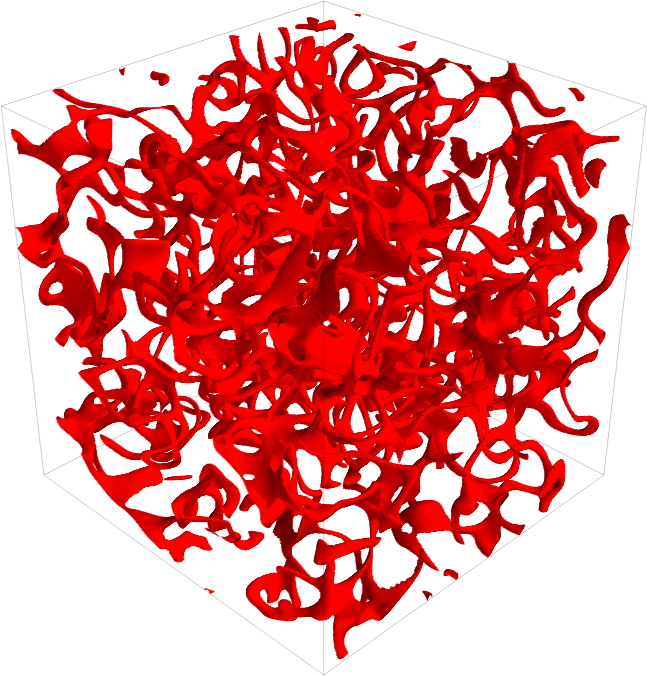
\includegraphics[width=0.25\linewidth]{nonequib/figures/IC/CF05-IC-t000}
    \raisebox{1.4in}{b)}~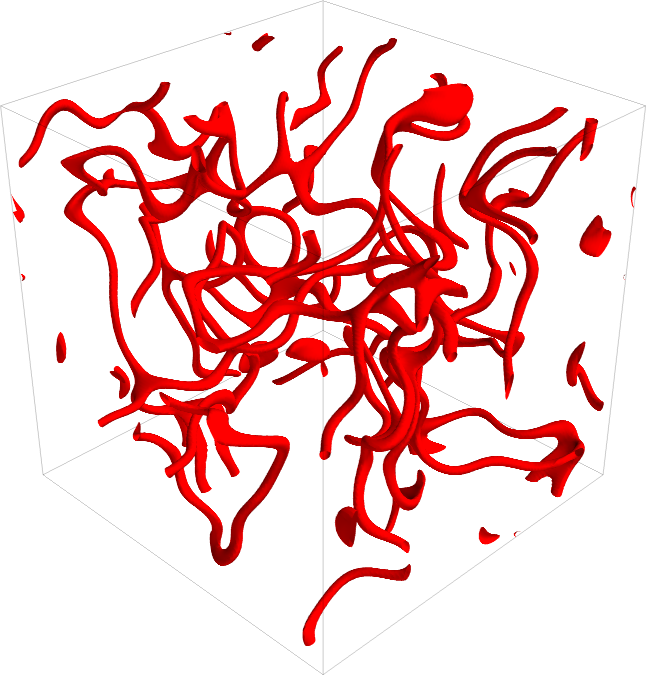
\includegraphics[width=0.25\linewidth]{nonequib/figures/IC/CF05-IC-t200}
    \raisebox{1.4in}{c)}~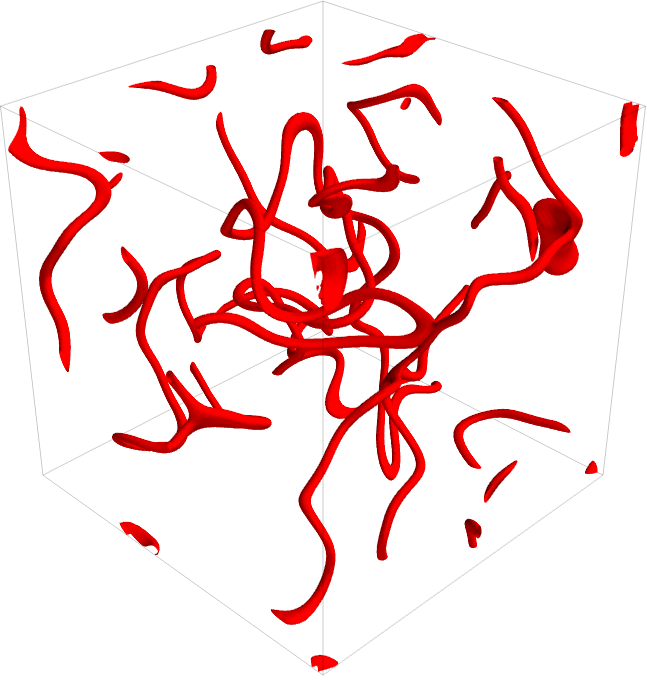
\includegraphics[width=0.25\linewidth]{nonequib/figures/IC/CF05-IC-t400}\\
    \raisebox{1.4in}{d)}~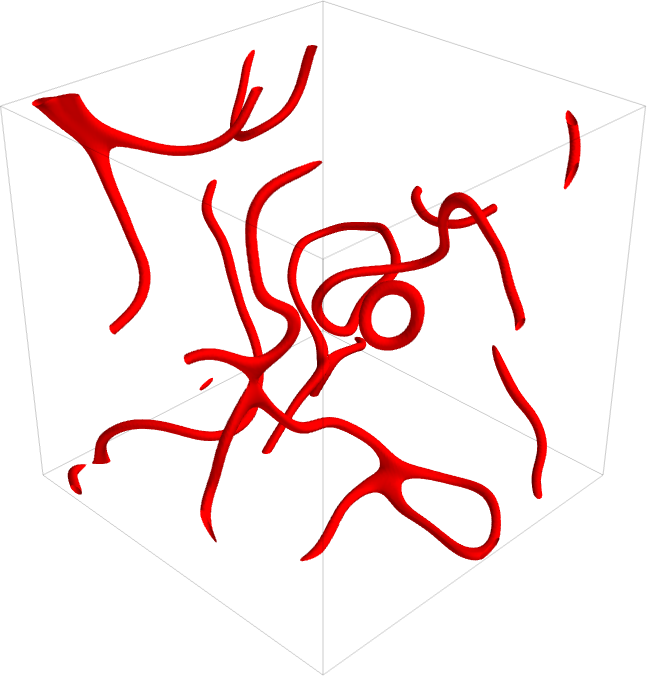
\includegraphics[width=0.25\linewidth]{nonequib/figures/IC/CF05-IC-t800}
    \raisebox{1.4in}{e)}~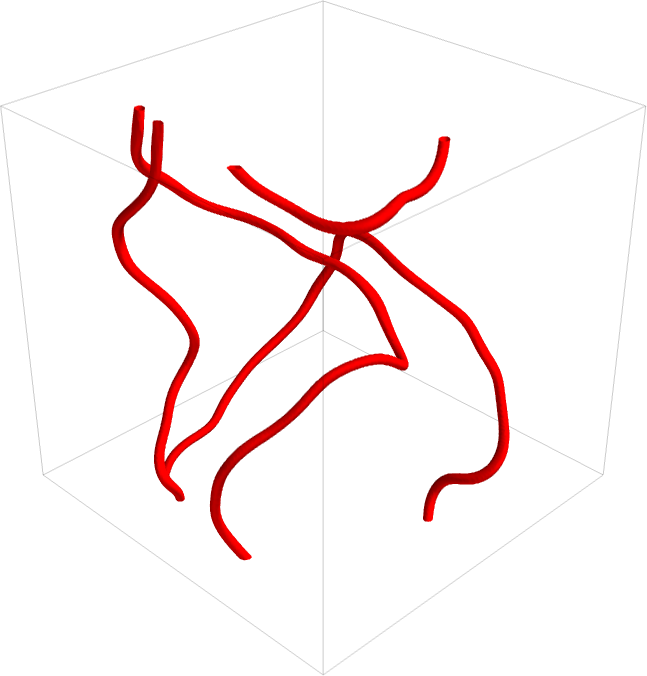
\includegraphics[width=0.25\linewidth]{nonequib/figures/IC/CF05-IC-t1600}
    \raisebox{1.4in}{f)}~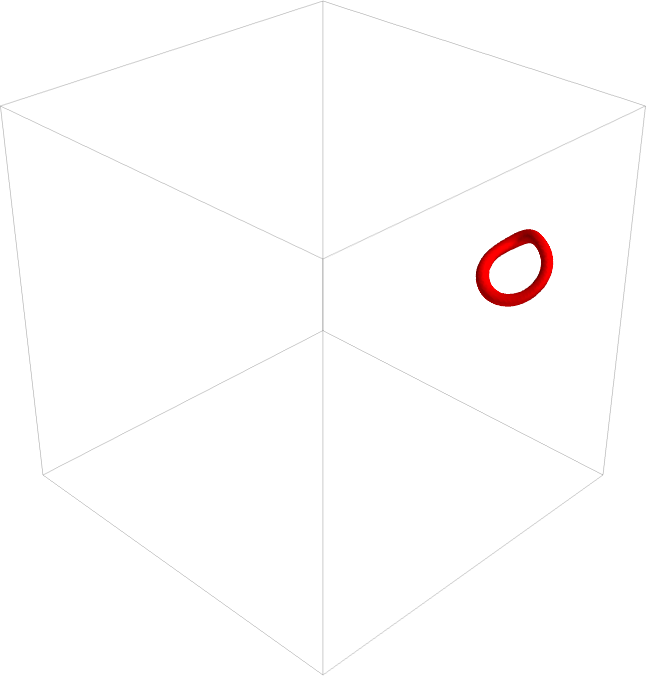
\includegraphics[width=0.25\linewidth]{nonequib/figures/IC/CF05-IC-t4000}
    \caption{(Color online) Evolution of the quasi-condensate vortex tangle during the equilibration dynamics at times (a) $t/\tau=0$, (b) $500$, (c) $1000$, (d) $2000$, (e) $4000$, and (f) $10\,000$.  Shown are isosurfaces of the quasi-condensate density $|\hat{\psi}|^2 = 0.04\braket{|\hat{\psi}|^2}$. At later times all vortices disappear.  Note that vortices cannot be visualized directly from the raw $\psi$ due to the significant thermal fluctuations.
%Here $\rho_0 = 0.5$,
}
    \label{fig:thermal}
\end{figure}


\begin{figure}
  \centering
    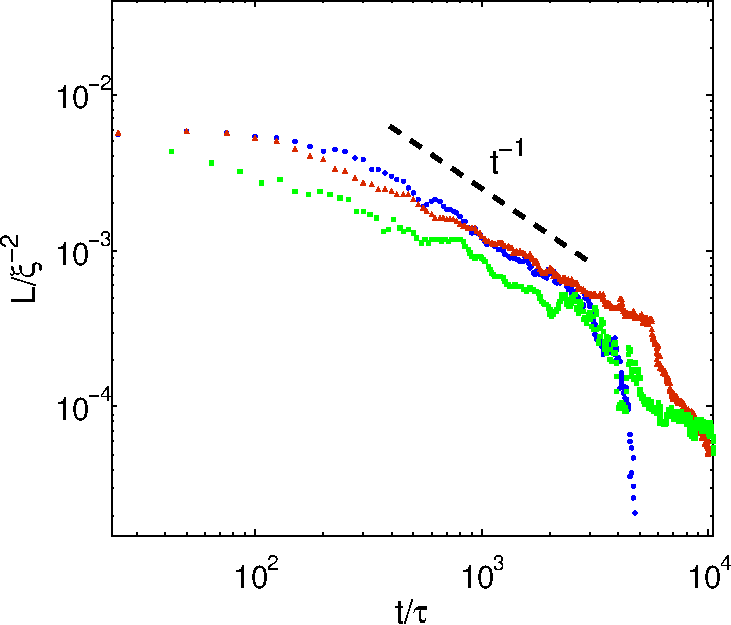
\includegraphics[width=0.45\linewidth]{nonequib/figures/ll_t_2}
    \caption{(Color online) 
Decay of the vortex line-length density during the equilibration dynamics, for various values of final condensate fraction:  $\rho_0/\rho = 0.2$ (blue circles), $\rho_0/\rho = 0.5$ (brown triangles) and $\rho_0/\rho = 0.9$ (green squares)
}
    \label{fig:ll_t}
\end{figure}




  \section{Moving obstacle at finite-temperature\label{sec:obstacle}}
\subsection{Set-up}
Having obtained the equilibrated finite-temperature states of the Bose gas, we now move on to consider a laser-induced obstacle moving through the gas.  The obstacle, uniform in $z$, is translated in the $x$-direction at speed $v$.  Our simulations are conducted in the frame moving with the obstacle, modelled by the inclusion of a Galilean shift term $i \hbar v \partial_x \psi$ to the right-hand side of the GPE.  In this frame the obstacle is imposed through the time-independent potential $V{(\bf r})=V_0 \exp\left[{-(x^2+y^2)/d^2 }\right]$, where $d$ and $V_0$ parameterize the width and amplitude of the potential.  We employ a fixed amplitude $V_0=5\mu$.   The frame speed is increased adiabatically to the required value according to the temporal profile $v \tanh(\hat{t}/200 \tau)$, where $\hat{t}$ denotes the time from introduction of the obstacle.

  
\subsection{Critical velocity \label{sec:vc}}
Simulations are repeated (from identical initial conditions) with increasing terminal speeds (in steps of $0.057c$) until vortices are observed to be nucleated from the obstacle (at an observation time of $\hat{t}=500\tau$). This defines the critical velocity $v_c$.  



Figure \ref{fig:vc-n0} shows the variation of $v_c$ with both condensate fraction $\rho_0/\rho$ (lower abscissa) and temperature $T/T_\lambda$ (upper abscissa), for two example obstacles widths.  The critical velocity has a maximum value at zero temperature (unit condensate fraction), and decreases nonlinearly as temperature increases (condensate fraction decreases), reaching zero at the critical point for condensation.  

At zero temperature, the critical velocity is of the order of the condensate speed of sound $c=\sqrt{\rho g/m}$, with a general form $v_{\rm c}(T=0)=\beta c$,
where $\beta$ is a parameter which depends solely on the shape of the obstacle (here $d$ and $V_0$).  The simulated $v_c$ data in Figure \ref{fig:vc-n0} closely follows a simple functional form given by $v_{\rm c}(T) = v_{\rm c}(T=0) \sqrt{\frac{\rho_0}{\rho}}$, as shown by the dashed lines.  Combining these forms, we can write a generalized form of the critical velocity, valid at zero and non-zero temperatures, as,
\begin{equation}
v_{\rm c}(T)=\beta \sqrt{\frac{\rho_0 g}{m}}.
\label{eqn:finite_vc}
\end{equation}
In other words, for a given obstacle, the critical velocity is a fixed ratio of the speed of sound based on the {\it condensate} density, rather than the total particle density \cite{leadbeater_2003}.  

The inset of Figure \ref{fig:vc-n0} shows the variation of $v_{\rm c}$ with the obstacle width $d$ at finite temperature, for the example of $T/T_\lambda =0.56$.   The qualitative behaviour is consistent with that seen at zero temperature \cite{huepe00,rica_2001,stagg_2014}: for small $d$ the critical velocity is sensitive to $d$ (due to the prominence of boundary layer effects) but as $d$ increases $v_c$ decreases towards a limiting values (the Eulerian limit).  However, the critical velocities are systematically reduced compared to the zero temperature case due to the reduced condensate speed of sound at finite temperature. 



\begin{figure}[h]
\centering
  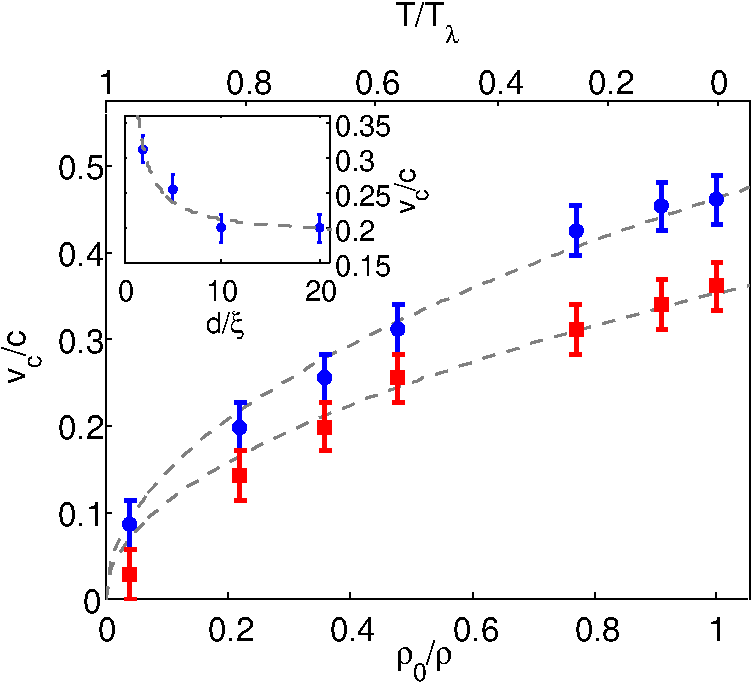
\includegraphics[width=0.45\linewidth]{nonequib/figures/vc-n0}
  \caption{\label{fig:vc-n0}(Color online) Critical velocity $v_{\rm c}$ for the moving Gaussian-shaped obstacle (uniform in $z$) as a function of condensate fraction $\rho_0/\rho$ and temperature $T/T_\lambda$, for obstacle widths $d=2\xi$ (blue circles) and $d=5\xi$ (red squares). The dotted lines show the analytic approximation $v_{\rm c}=\beta \sqrt{\rho_0/\rho}$ with fitted coefficients $\beta=0.46$ and $0.35$. (Inset) The critical velocity approaches an asymptotic value as the obstacle size is increased. Included is a fit of the form $v_{\rm c}=\alpha/d+\gamma$ with $\alpha=0.26~(\xi^2/\tau)$ and $\gamma=0.18 c$.  Errors bars arise from the discretized values of $v$ considered.}
\end{figure}

\subsection{Vortex nucleation}

Finally we examine the manner in which vortices are nucleated from the obstacle.  At zero temperature, one expects the nucleation of straight anti-parallel vortex lines from the obstacle, either released in unison or staggered in time \cite{saito_2010,stagg_2014}, and move downstream relative to the obstacle.  Pairs of anti-parallel quantized are unstable to sinusoidal perturbations - the Crow instability - which grow over time, and may eventually lead to the lines reconnecting and generating vortex rings \cite{berloff_2001,simula_2011,zuccher_2012}.  However, in the zero temperature case, this instability is very slow to manifest on a visible scale due to the high degree of parallelism of the vortex lines.  Numerical simulations speed up the instability by imposing an initial perturbation on the vortex line, and the instability may be naturally sped up in an inhomogeneous condensate, where the vortex lines naturally deviate from straight lines.

We find two qualitative regimes of vortex nucleation at finite temperature.  The first case is illustrated through the example in Fig.  \ref{fig:vort-lines}.  A pair of ``wiggly'' vortex lines are nucleated from the obstacle, as seen in the final snapshot (iv).  The wiggles are drive by the thermal fluctuations, which cause the vortex elements to be nucleated at slightly different times along the obstacle; this is visible at intermediate times (snapshots (iii) and (iv)).   This regime of nucleation tends to occur for low speeds.

\begin{figure}
		\centering
    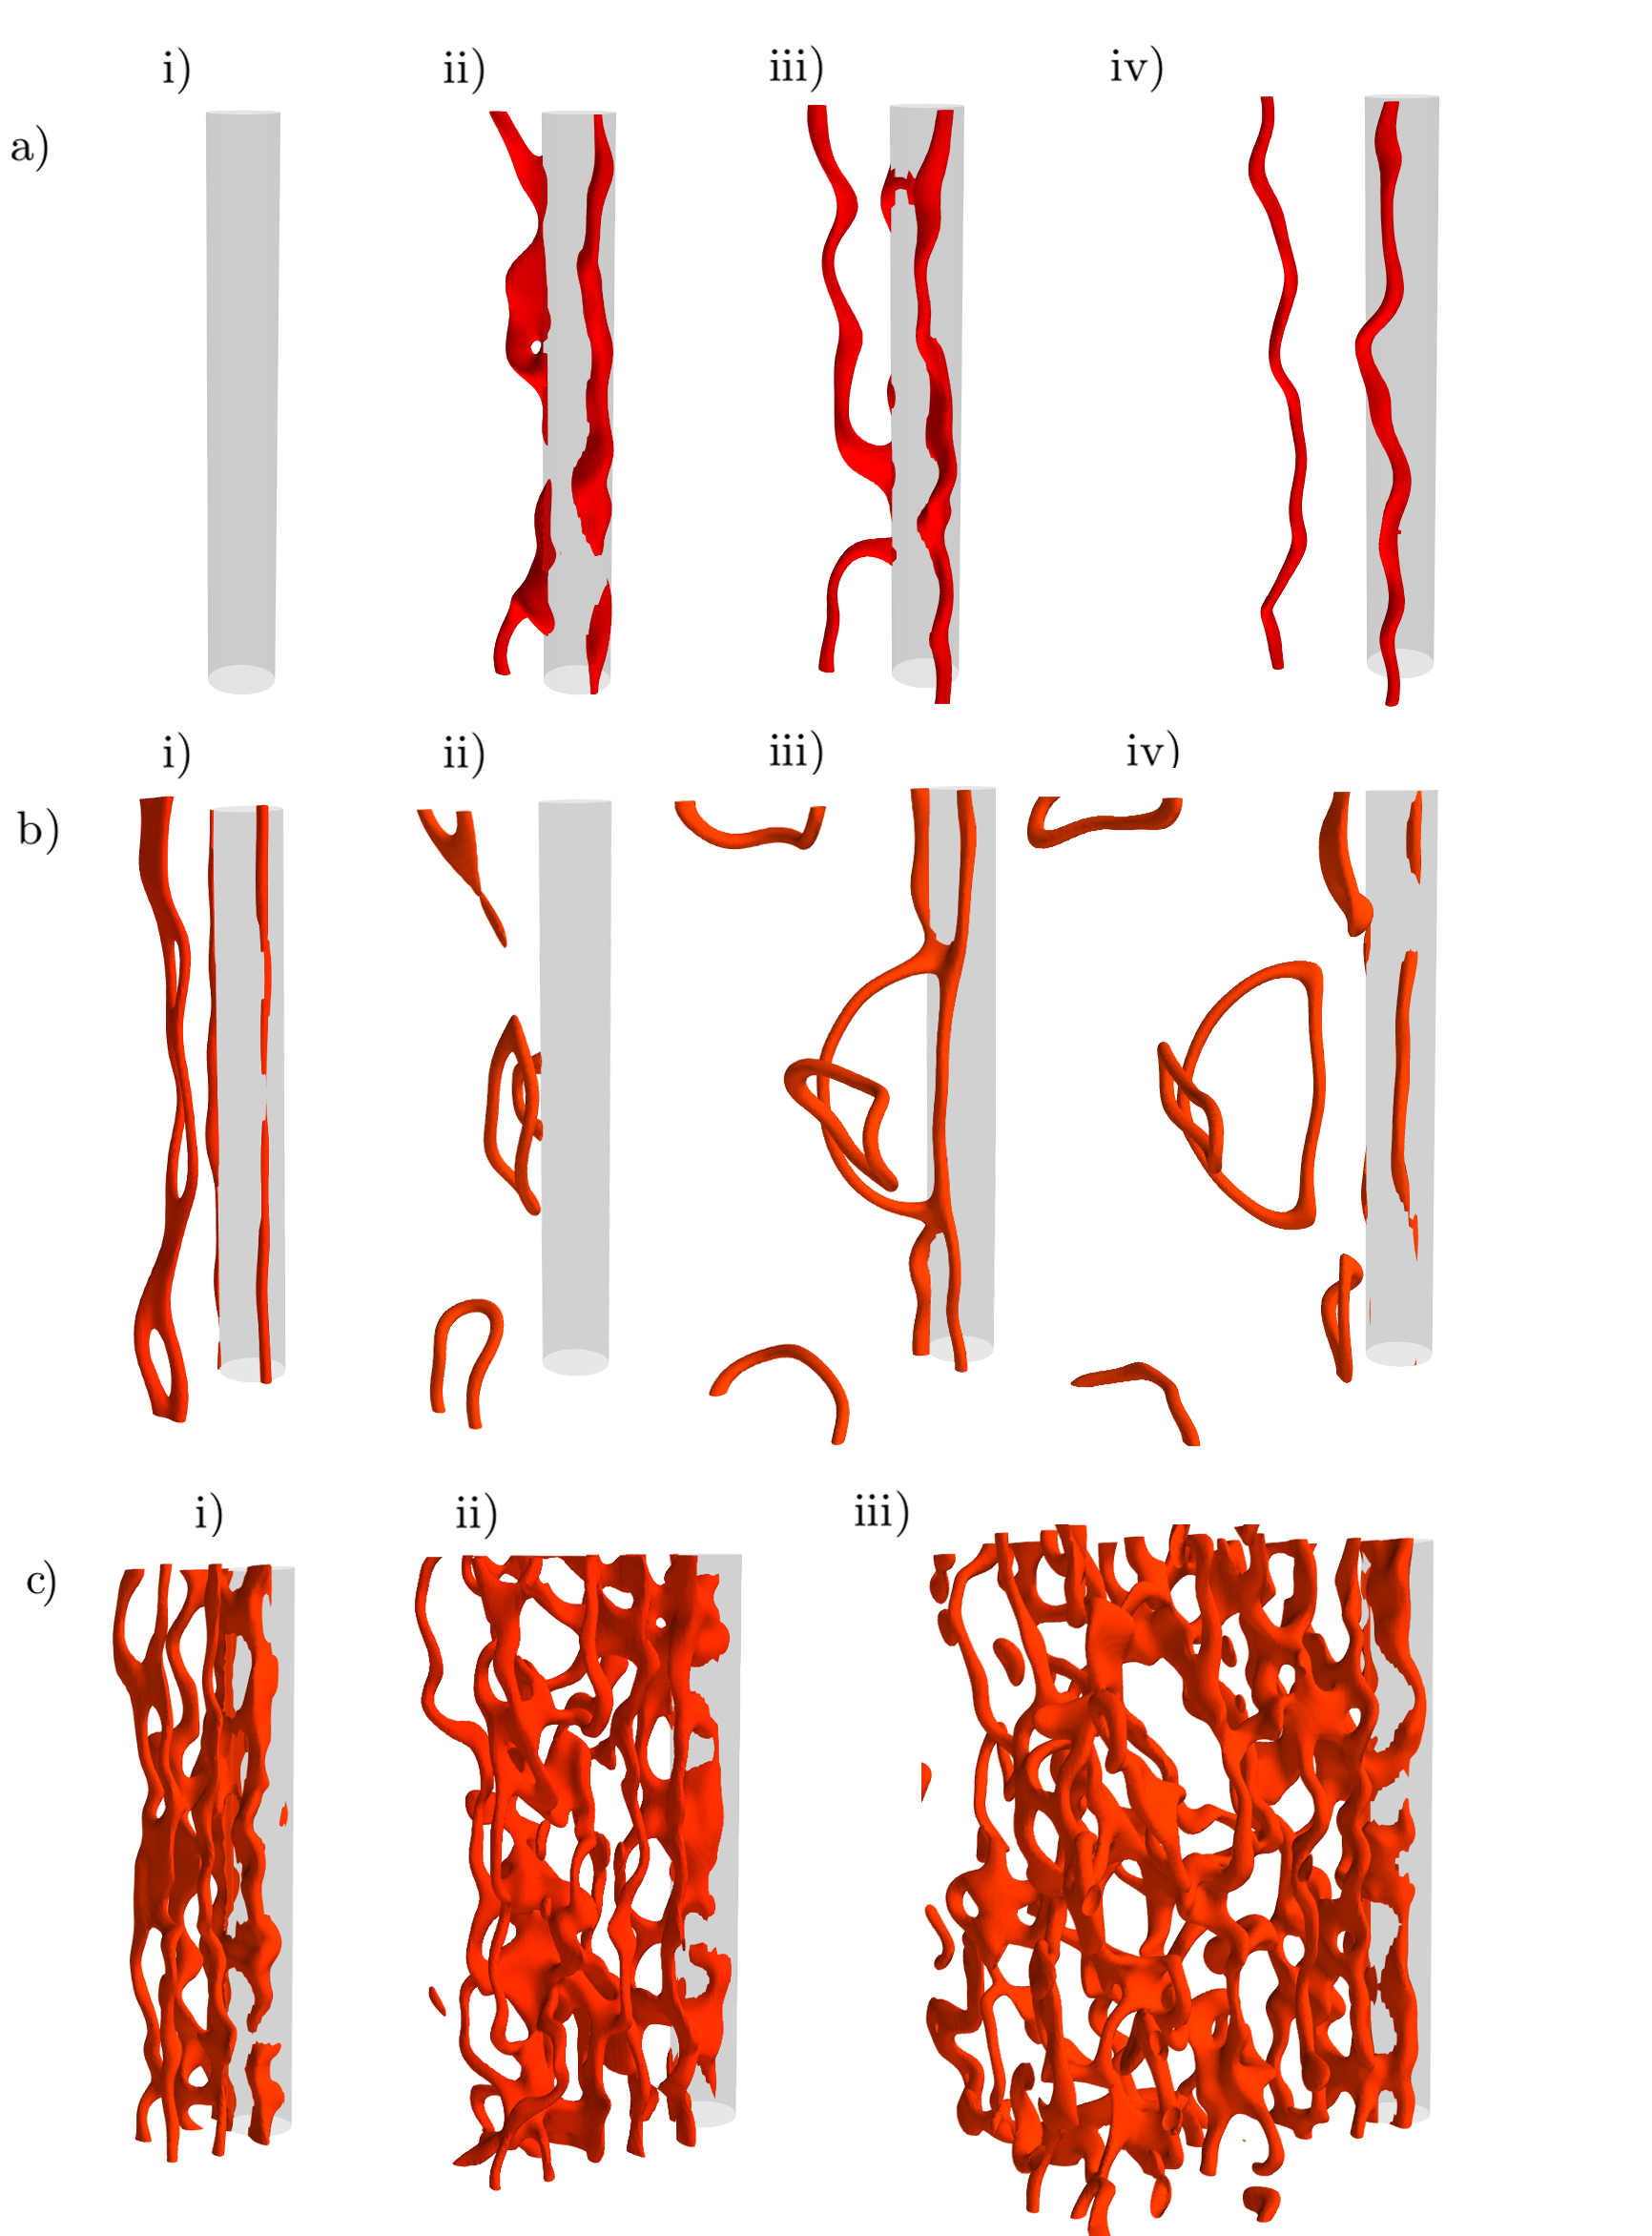
\includegraphics[width=0.6\linewidth]{nonequib/figures/vort}
    \caption{\label{fig:vort-lines}(Color online) Snapshots of the typical vortex nucleation from the moving Gaussian-shaped obstacle (gray) in the finite temperature Bose gas.  Shown are  isosurfaces of the quasi-condensate density ($|\hat{\psi}|^2 = 0.04\braket{|\hat{\psi}|^2}$).  (a) Vortices are shed as pairs of anti-parallel vortex lines.  Here the system parameters are $\rho_0/\rho = 0.2$ and $v=0.17c$, and the snapshots correspond to times (i) $\hat{t}/\tau=210$, (ii) $460$, (iii) $585$ and (iv) $710$.   (b) Vortex rings are nucleated from the obstacles.  The system parameters are $\rho_0/\rho = 0.9$ and $v=0.37c$, and the times are (i) $\hat{t}/\tau=0$, (ii) $125$, (iii) $250$ and (iv) $500$.}
\end{figure} 


Figure \ref{fig:vort-lines}(b) shows an example of the second regime of nucleation, which is characterised by the emission of vortex rings, rather than lines.  This behaviour occurs for larger speeds.  Again, the thermal fluctuations induce vortex nucleation at different times along the obstacle, but now the enhanced speed causes these localized vortex loops to peel away significantly from the obstacle, forming a series of vortex rings.   
At even higher speeds ($v/v_{\rm c} \gg 1$), the frequency of vortex nucleation is large, with a significant interaction between successively-nucleated vortices.  This leads to a complex tangle of vortex lines behind the obstacle. 

\section{Conclusions\label{sec:conclusions}}
Using classical field simulations we have analysed the nucleation of vortices past a moving cylindrical obstacle in a finite temperature homogeneous Bose gas. We evolve the classical field from highly non-equilibrium initial conditions to thermalized equilibrium states with ranging temperatures and condensate fractions.  During this evolution, the vortex tangle present in the quasi-condensate is shown to decay in accord with the Viven/ultraquantum form.  A cylindrical obstacle with Gaussian profile is then introduced into the system, and the gas made to flow relative to the obstacle.  Above the critical velocity, vortices are nucleated, either as wiggly anti-parallel pairs of vortex lines or as vortex rings. The critical velocity decreases with increasing temperature, becoming zero at the critical temperature, and scales with the speed of sound of the condensate, i.e. as the square root of the condensate fraction.  
\end{chapter}
